\documentclass[12pt, a4paper, onecolumn]{article}


%package pour rétrécir les marges
\usepackage[margin=64pt]{geometry}

%package pour les équations mathématiques
\usepackage{amsmath}

%package pour les tableaux (pour l'annexe 1)
\usepackage{array}

%package et commande pour les alinéas
\usepackage{tabto}
\renewcommand{\tab}{\tabto{15px}}

%pacakges pour la bibliographie
\usepackage[toc,page]{appendix}
\usepackage{hyperref}
\usepackage[super]{natbib}

%package pour le signe €
\usepackage{eurosym}

%package pour les couleurs (utiles pour les références)
\usepackage{xcolor}

%packages pour les graphes (conversions eps -> pdf et affichage)
\usepackage{graphicx}
\usepackage{epstopdf}
\usepackage{subfigure}
\usepackage{float}

%packages pour rajouter des sous-sous-titres
\usepackage{titlesec}
\usepackage{scrextend}
\usepackage{changepage}
\setcounter{secnumdepth}{3}

%commande permettant de citer plusieurs sources à la fois (le package permet la création de la fonction récursive)
\usepackage{etoolbox}
\makeatletter
\newcommand{\csvdel}{}
\newcommand{\bettercite}[1][,]{%déclaration de la fonction générale
  \renewcommand{\csvdel}{\renewcommand{\csvdel}{}}%lors de l'appel commence par rajouter un crochet
  \csname\endcsname$^[$\checknextarg}
\newcommand{\checknextarg}{\@ifnextchar\bgroup{\gobblenext}{}}%vérifie si un autre argument existe
\newcommand{\gobblenext}[1]{\csvdel\textcolor{blue}{\textbf{\cite{#1}}}\@ifnextchar\bgroup{$^,$\gobblenext}{$^]$}}%récupère l'argument qui suit, met la source et une , s'il existe sinon ferme le crochet
\makeatother

%commande pour mieux citer les annexes et figures/images
\newcommand{\cfannexe}[1]{\textsuperscript{(\textcolor{blue}{\textbf{\ref{annexe #1}}})}}
\newcommand{\cffig}[1]{\textsuperscript{\{\textcolor{blue}{fig.\textbf{\ref{#1}}}\}}}

%packages et commandes pour surligner le numéro de la figure
\usepackage{ulem}
\usepackage{caption}[2007/09/01] % needs v3.1 or newer
\DeclareCaptionLabelFormat{underlcap}{\uline{#1 #2}}
\captionsetup[figure]{labelformat=underlcap}

%Evite l'apparition de traits d'unions pour séparer les mots sur plusieurs lignes
\tolerance=1
\emergencystretch=\maxdimen
\hyphenpenalty=10000
\hbadness=10000



%définition du titre des auteurs et autres informations clé
\title{Performance comparison between maglev and current rail technologies}
\author{Mathieu Denglos, Kerian Chauvin}
\date{}



\begin{document}


%page 1
\maketitle  %titre

\begin{figure}[H] %image d'introduction
  \centering
  \scalebox{0.28}
  {\includegraphics{img/image_couverture.png}}
\end{figure}



\pagebreak %page 2
\section*{Abstract} %Résumé
\tab With the ecological matters becoming more and more important in the last few years, the different governments are turning to rail transport because it is more ecological.
However, trains are not the only guided vehicles with a strong potential in terms of ecology and performance.
The media regularly talks about maglev technologies as very fast vehicles with a great potential.\\
\tab To compare this high potential, it is essential to take into account all the technical aspects that characterize the performance of the system.
However, the studies already conducted on maglev vehicles rarely compare these two systems, and generally only on specific points. \\
\linebreak
\tab That is why we have decided, in the same study, to group together an objective comparison of these different technical characteristics, in order to determine the potential benefits of maglev technologies over those of trains, and in which cases it is judicious to move towards one technology or another. \\
\linebreak
\tab Contrary to what the general public may think about maglev technologies, the technical capabilities evoked in the media are not generalized to all maglev.
The combination of our results also allows us to conclude that no single technology stands out and that, depending on the route or technical constraints, a case-by-case study is necessary to determine which technology would be the most appropriate. \\

\section*{Introduction} %Introduction
\tab Maglev vehicles are often shown in the media and in the collective imagination as the guided transport of the future, with phenomenal speeds.
In truth, such a conclusion is not directly possible.
These technologies are far more complex and subtle than one might think.
To an outsider, maglev vehicles and trains are very similar.
Their structures are similar, the only notable difference being the wheel-rail contact, which is missing on the maglev and replaced by levitation technologies. \\
\linebreak
\tab Ces différents aspects nous amènent à nous demander ce qui peut différencier les technologies maglev avec celles des trains, principalement sur leurs performances, tout en se questionnant sur l’influence du contact roue-rail. \\
\tab These different aspects lead us to ask what can differentiate maglev technologies from train technologies, mainly on their performances, while questioning the influence of the wheel-rail contact. \\
\linebreak
\tab It is important to mention that throughout this study, projects such as the hyperloop will not be mentioned because, as they travel at reduced pressure, the aerodynamic drag is strongly reduced (up to 10 times)\bettercite{maglevintube}, distorting the potential results collected.
Moreover, we will only focus on catenary-powered electric railcars in the case of trains, to be as close as possible to maglev vehicles. \\



\pagebreak %page 3
\section{Presentation of the technologies studied} %Partie 1 : technologies étudiées
\tab In contrast to the relatively standardized systems of modern railways, maglev systems are multiple and each has its advantages and disadvantages.
Because of the number of studies and open lines, two propulsion technologies are of particular interest:
\begin{itemize}
  \item LIM propulsion using short stator (Linear Induction Motor),
  \item LSM propulsion using long stator (Linear Synchronous Motor).
\end{itemize}
\tab Before answering our problem, it is important to detail the functions of these various little known technologies.

\subsection{Train technologies}
\tab The operation of trains is based on a 5 centuries old technology, the guidance of a wheeled vehicle by the use of rails. \\
\tab Electric railway traction by catenary is first of all made possible by a continuous or single-phase power supply.
After various transformations using choppers, rectifiers or inverters, this power is fed to the train motors. \\
\linebreak
\tab There are three types of electric motors used in railways: the direct current motor, the synchronous motor and the asynchronous motor. \\
\tab The DC motor receives a DC power supply.
The stator, when powered, will create a magnetic field within it and thus allows the rotor within it to rotate. \\
\tab  The stator of synchronous and asynchronous motors receives a three-phase power supply, with the three phases feeding the three coils of the stator, creating a rotating field.
In the case of a synchronous motor, the rotor, consisting of a permanent magnet or a coil supplied with direct current, will follow this field and thus be driven in rotation.
In the case of an asynchronous motor, the rotor is made up of closed and independent turns which will be the seat of induced currents when the rotor is subjected to the rotating field.
They will then drive it in rotation by trying to catch this field. \\
\tab These motors then drive the driving axles of the train and thus set it in motion.
This is made possible by the adhesion, albeit weak, between the wheel and the rail, the main difference between the train and maglev vehicles.

%Images train
\begin{figure}[H]
  \centering
  \begin{minipage}{0.5\textwidth}
    \includegraphics[width=\textwidth]
    {img/adherence.jpg}
    \caption{representation of the wheel-rail contact}
    \label{adherence}
  \end{minipage}\hfill
  \begin{minipage}{0.5\textwidth}
    \includegraphics[width=\textwidth]
    {img/bogietrain.png}
    \caption{bogie of the tgv}
    \label{bogietrain}
  \end{minipage}
\end{figure}



\pagebreak %page 4
\subsection{LIM and EMS technologies}
\tab The maglev with linear induction motor (LIM) technology is the first of the two technologies currently deployed.
Like any motor, the LIM consists of two parts: the rotor, located under the vehicle and being the powered part of the motor, and the stator composed of a steel plate on aluminum, located on the rail.
The rotor, located on the train is powered and will generate a magnetic field parallel to the rotor.
This magnetic field will induce a current in the rail (according to Lenz's law) which itself will generate a magnetic field parallel to the stator (thus to the rotor) and in the opposite direction to the rotor.
These two magnetic fields oppose each other, pushing back the rotor and making the train move forward\bettercite{coloradomaglev}\cffig{schemaLIM}. \\
\linebreak
\tab The motorization is not the only technical aspect to study in order to answer our problem.
The technology of levitation is also impacting on the performance of the vehicle.
In the case of LIM maglevs, it is the electromagnetic levitation (EMS) which is most commonly used.
The EMS technology consists of two series of electromagnets attached to the vehicle and located under the rail for levitation, and on the sides for guidance\cffig{schemaEMS}.
When these are powered, they are attracted by the rail, levitating the train from below for the levitation magnets and allowing the stability of the vehicle for the guidance magnets.
Sensors are located around the levitation magnets, allowing, by regulating the power sent in the electromagnets, to keep a constant distance between the LIM and the rail (generally 8 $\pm$ 3mm\bettercite{koreamaglevprogram}). \\

\begin{figure}[H]
  \centering
  \begin{minipage}{0.45\textwidth}
    \includegraphics[width=\textwidth]
    {img/schemaLIM.png}
    \caption{LIM operating diagram}
    \label{schemaLIM}
  \end{minipage}\hfill
  \begin{minipage}{0.45\textwidth}
    \includegraphics[width=\textwidth]
    {img/schemaEMS.png}
    \caption{EMS operating diagrame}
    \label{schemaEMS}
  \end{minipage}\par
  \vskip\floatsep% normal separation between figures
  \includegraphics[width=0.68\textwidth]
  {img/bogieLIM.png}
  \caption{bogie of the Changsha maglev express\bettercite{changshasources}}
  \label{bogieLIM}
\end{figure}



\pagebreak %page 5
\subsection{Technologies LSM et EDS}
\tab The other technology developed is the maglev synchronous linear motor (LSM) technology.
Like the LIM, the LSM is divided into two parts, the rotor and the stator.
However, its operation is totally different from that of the LIM.
The rotor (located on the train) consists of permanent magnets with alternating polarity (N,S,N,...). The stator (located on the rail) is composed of electromagnets with alternating polarity.
This technology uses the fundamental principle of magnets that attract each other when their polarities are opposite.
When the rail electromagnets are energized, they behave like magnets, and therefore attract the poles of the train magnets.
However, as soon as the poles are opposite, the train should stop, so we change the direction of the current in the coils, to reverse the poles of the electromagnets.
The south pole of the train is then attracted by a new north pole a little further along the rail, and so on all along the route\bettercite{coloradomaglev}\cffig{schemaLSM}. \\
\linebreak
\tab For the levitation, the LSM systems are associated with an electrodynamic levitation (EDS).
This, unlike the EMS system, uses the principle of repulsion of magnets of the same polarity.
The track includes, in addition to the coils for the linear motor, coils to levitate the train.
This system is usually located under the train, or on the sides\cffig{schemaEDS} such as on the Chuo Shinkansen line.
Unfortunately, this system is not sufficient as it only works on medium and high speeds (over 100km/h).
To meet the needs of low speeds, the EDS technology is combined with an EMS system or wheels\bettercite{maglevtech}.
Finally, some lines combine levitation with superconductivity (bringing the system to very low temperatures) to improve performance.

\begin{figure}[H]
  \centering
  \begin{minipage}{.51\linewidth}
    \includegraphics[width=\textwidth]{img/schemaLSM.png}
    \caption{LSM operating diagram}
    \label{schemaLSM}
  \end{minipage}
  \begin{minipage}{.48\linewidth}
    \includegraphics[width=\textwidth]{img/voirie.png}
    \caption{tracks elements}
    \label{schemaEDS}
    \includegraphics[width=\textwidth]{img/bogieLSM.jpg}
    \caption{MLX-01 bogie (Chuo Shinkansen)}
    \label{bogieLSM}
  \end{minipage}
\end{figure}



\pagebreak %page 6
\subsection*{Functional comparison of these technologies}

\tab Although these two maglev technologies will be studied on the same points in order to answer our general problem, it is still important to determine which one is closer to the train, which will allow us to focus on our secondary problem of the impact of the wheel-rail contact on performance.
The best way to find the maglev technology that is closer to the train without going into technical data is to compare their traction chain. \\

\begin{figure}[H]
  \centering
  \begin{minipage}[H]{0.47\textwidth}
    \includegraphics[width=\textwidth]{img/CTCtrain.png}
    \;(a) continuous lotor train
  \end{minipage}
  \hfill
  \begin{minipage}[H]{0.47\textwidth}
    \includegraphics[width=\textwidth]{img/CTCLIM.png}
    \;(b) LIM maglev
  \end{minipage}\par
  \vskip\floatsep\par
  \vskip\floatsep

  \begin{minipage}[H]{0.47\textwidth}
    \includegraphics[width=\textwidth]{img/CTAtrain.png}
    \;(c) synchronous/asynchronous motor train
  \end{minipage}
  \hfill
  \begin{minipage}[H]{0.47\textwidth}
    \includegraphics[width=\textwidth]{img/CTALSM.png}
    \;(d) LSM maglev
  \end{minipage}
  \caption{Traction chains}
\end{figure}

\tab By comparing the above traction chains, we can see that the LIM propulsion technology is the closest to the continuous motor train.
This is logical because the overall operation remains similar compared to our current trains, the only notable difference coming from the wheel-rail contact which generates the need to convert the rotary motor into a linear motor. \\
\linebreak
\tab The traction chain of the LSM propulsion is totally different from that of the current trains.
In this case, the difference found is also logical because LSM technologies do not require any internal power system in the train, except for the auxiliary elements (light, heating...).
Indeed, most of the propulsion is located on the rail itself.
Nevertheless, we have brought a strong interest to this technology because it will allow us to question the generalized vision of maglev systems with the results we have found.\\



\pagebreak %page 7
\section{Selection criteria}

\tab Our objective is to compare the two maglev technologies to those of trains. We will compare them on three main axes :
\begin{itemize}
  \item The journey: comparison of the different parameters influencing the journey times,
  \item The cost: destination of investments at different moments in the life of a line,
  \item Other criteria that may influence the choice of network type.
\end{itemize}

\subsection{Journey}
\tab When analyzing a transportation system, the most important characteristic from the user's point of view is the travel time.
This is mainly influenced by the speed of the train, but also its acceleration and deceleration capabilities.

\begin{addmargin}[30px]{0px} \subsubsection*{Speed}\end{addmargin}
\tab Let's start by recalling the maximum commercial speeds of trains running on the different rail networks today. These are generally limited to between 320 km/h and 360 km/h for high-speed lines. \\
\tab In the media, maglev vehicles are always portrayed as much faster technologies; however, a distinction must be made between the two technologies because the results vary greatly. \\
\linebreak
\tab Starting with LIM propulsion technology, we find results that are much lower than those stated for trains and in opposition to the general public's vision.
Indeed, the maximum commercial speeds on open lines never exceed 120km/h\cfannexe{1}.
Further research has shown that even if this technology were optimized, speeds would remain around 160 km/h\bettercite{optimisationchangsha}. \\
\linebreak
\tab It is by researching LSM technologies that the results seem much more interesting.
Indeed, the speeds reached with this rolling stock exceed 400 km/h for classical EDS levitation technologies and can be pushed up to 550-600 km/h for EDS coupled with superconductivity\cfannexe{1}. \\
\linebreak
\tab Although for any type of transportation, speed is an important point, in the context of a guided system, safety remains paramount and is the first point taken into consideration when implementing systems.
The speed is an important point to watch because the risk of instability and therefore of derailment increases strongly with the speed.
In order to justify the above mentioned results, it is important to look at the speeds where the instability becomes too important, also called critical speed.
\pagebreak  % Page 8
These critical speeds can be influenced by different factors, controllable or not by the manufacturer.
To increase it, the manufacturer can for example decrease the mass of the bogie or improve the stabilization devices.
It is therefore important to understand that these results are impacted by the chosen rolling stock and that the results expressed above cannot take into account all situations. However, in the case of our study, orders of magnitude are sufficient to draw a conclusion about the impact of the different technologies on the critical speed. \\
\linebreak
\tab For trains currently in service, depending on the countries and conditions mentioned above, the value varies between 430 km/h (for softer ground) and 580 km/h (for harder ground)\bettercite{vitessecritiquetrain}.
Knowing that in addition to the points mentioned above, the railway manufacturers play on other parameters to improve the stability of the bogie such as the wheelbase (which can reach 3 meters for the TGV) and the conicity of the wheels. \\
\linebreak
\tab For LIM technologies, the critical speed is low, around 250 km/h\bettercite{vitessecritiquelim} for a gap of 8mm between the motor and the rail (the most common gap found) and is proportional to it. \\
\tab This is not directly induced by the propulsion technology, but mainly by the lift technology.
Indeed, the EMS levitation technologies require a very precise spacing (within a few millimeters), spacing which can be difficult to maintain at high speed and which increases the risks of accidents. \\
\linebreak
\tab For LSM technologies, the critical speed is complicated to calculate because it depends on many variables that can drastically change the result.
However, to give a broad range taking into account the conditions of use, the critical speed for LSM systems is between 700 km/h and 900km/h\bettercite{vitessecritiquelsm}. \\
\tab Contrary to the EMS levitation which becomes quickly unstable, the EDS levitation technologies which are linked to the LSM propulsion remain stable even at very high speeds, moreover, the use of superconductivity improves the global stability even more, and thus allows higher speeds.\\
\linebreak
\tab With this information, we can already conclude about the potential traction programs that each technology can achieve.
Indeed, the traction programs of high-speed trains and maglev LSM technologies can perfectly fit the needs for long distances thanks to their high speeds, while LIM technologies which have limited speed capabilities will be suitable for shorter distance networks, such as metros, VAL or Regional Express Networks.
Although the traction program depends on more factors, our assumptions are confirmed when we look at the routes taken by the existing lines\cfannexe{1}. \\

\begin{addmargin}[30px]{0px} \subsubsection*{Acceleration and deceleration}\end{addmargin}
\tab Although speed is a major factor in travel time, it is not the only factor influencing travel time.
The ability to accelerate and decelerate can also greatly improve this point. \\
\linebreak
\tab The acceleration and deceleration capacity of the train is one of its major shortcomings, caused mainly by the poor adhesion of the wheel-rail contact.
According to SNCF network figures, the minimum deceleration imposed for passenger trains is 0.5m/s² for a speed lower than 160km/h and 0.6 m/s² for a speed higher than 160 km/h\bettercite{decelerationtrain}.
For LIM, acceleration is between 0.9 and 1.1 m/s² and deceleration is 1.1 m/s² and reaches 1.3m/s² in case of emergency braking\bettercite{changshadata}{incheonairport}{linimo}.
For LSM, deceleration and acceleration is at 1.6m/s² and reaches up to 2.4m/s² in case of emergency braking\bettercite{maglevus}.\\
\tab As for any system, the acceleration of guided vehicles can be expressed using Newton's first law.
For guided vehicles, the Newton's first law is simply written \\
$$kM\gamma = R_{traction} - R_{r\acute{e}sistant}$$
\newpage%page 8
\tab Therefore, there are three factors that can increase the value of the acceleration:
\begin{itemize}
  \item the increase of the traction effort,
  \item the reduction of the resistant effort,
  \item the decrease of the mass.
\end{itemize}
\tab The increase in tractive effort will not be studied here because it varies drastically depending on the associated traction program\cfannexe{2}.
However, it is possible to increase it by adding motorization or by improving its power.
However, this decision has a strong impact on the transported mass and cost. \\
\linebreak
\tab The resisting force is generated by the resistance to the vehicles' advance as well as by the profile of the track. We then have :
$$R_{r\acute{e}sistant} = R_{av} + R_p$$
Since the resistance R$_p$ depends only on the track profile (gradient and/or curvature) and not directly on the propulsion technology, it will be considered null in this part.
As for the forward resistance, we have a quadratic equation depending on the speed and the shape of the vehicle :
$$R_{av} = A + BV + CV^2$$
\tab At high speeds (between 320 and 360 km/h), the range of interest, the A and BV terms are negligible.
According to the measurements made on different trains and maglev vehicles, the values of drag found are in the same order of magnitude\bettercite{ei}, showing a certain constancy of the C coefficient. \\
\tab Indeed, the aerodynamic coefficient C characterizes the air penetration of the vehicle.
It is therefore independent of the propulsion technology.
Coefficient A depends on the mechanical resistance, in particular the mass of the bodies, while coefficient B depends much more on the propulsion technology and corresponds to the other parameters of the vehicle, in particular its power, the wheel-rail contact in the case of trains or the resistance generated by the engine in the case of maglev.
The B coefficient is thus the one that differs the most between the technologies\bettercite{thesetgv}{ei}. \\
\tab The dynamic drag caused by the wheel-rail contact of the trains represents only 10 \% of the resistance to forward motion\bettercite{maglevintube}, hence the small difference in resistive forces. \\
\linebreak
\tab  The decrease in mass is the most obvious point.
In order to compare the mass of the vehicles according to their propulsion modes, we use here the mass per unit area (in kg/m²) as well as the length of the vehicles.
By using the formula $\sigma = \frac{m}{S}$ for each of the 3 propulsion modes studied, and taking the average value on the different lines studied, we find the following results for the technologies with regional services:
\begin{itemize}
  \item $\sigma_{train} = 660kg/m^2$
  \item $\sigma_{LIM} = 530kg/m^2$\bettercite{koreamaglevprogram}{changshadata}{linimo}
\end{itemize}
For intercity services :
\begin{itemize}
  \item $\sigma_{train} = 830kg/m^2$\bettercite{thesetgv}
  \item $\sigma_{LSM} = 650kg/m^2$\bettercite{ei}
\end{itemize}

\tab These results are not surprising considering the technologies involved.
As the propulsion technologies of regional and LIM trains are relatively close, their mass per unit area are logically close too.
The LSM vehicles stand out from the trains because of their lower mass per unit area due to the absence of propulsion technologies in the train itself, which are concentrated on the track.
In addition, maglev vehicles remain shorter than trains.
With 30m to 50m length for LIM vehicles and 80m to 120m length for LSM vehicles against 200m (in single unit) to 450m (in multiple unit) length for the train. \\
\linebreak
\tab Overall, these different points are in favor of maglev technologies, which remain much more efficient on their acceleration and deceleration compared to trains. \\
\tab However, in order to relate to the travel time, we will relate to the travel time.
It is with this in mind that we are going to look at the time lost by these different technologies during a station stop.
We will consider here only the commercial values and not the emergency braking values, as well as a zero stop time.
In order to calculate the lost time, we use the formula: \\
$$t_{perdu}(V) = t_{d\acute{e}c\acute{e}l\acute{e}ration}(V) + t_{acc\acute{e}l\acute{e}ration}(V) \; – \; \frac{d_{parcourue}(V)}{V}$$
\noindent With :
\begin{itemize}
  \item $t_{perdu}(V)$ : the time that the vehicle loses to stop from a speed V and to come back to this speed (example: during a stop in a station),
  \item $t_{d\acute{e}c\acute{e}l\acute{e}ration}(V)$ : the time it takes the vehicle to go from speed V to 0 km/h,
  \item $t_{acc\acute{e}l\acute{e}ration}(V)$ : the time it takes the vehicle to go from 0 km/h to speed,
  \item $d_{parcourue}(V)$ : the theoretical distance that the vehicle would have covered at constant speed during the deceleration/acceleration phase.
\end{itemize}

\begin{figure}[H]
  \centering
  \scalebox{0.48}
  {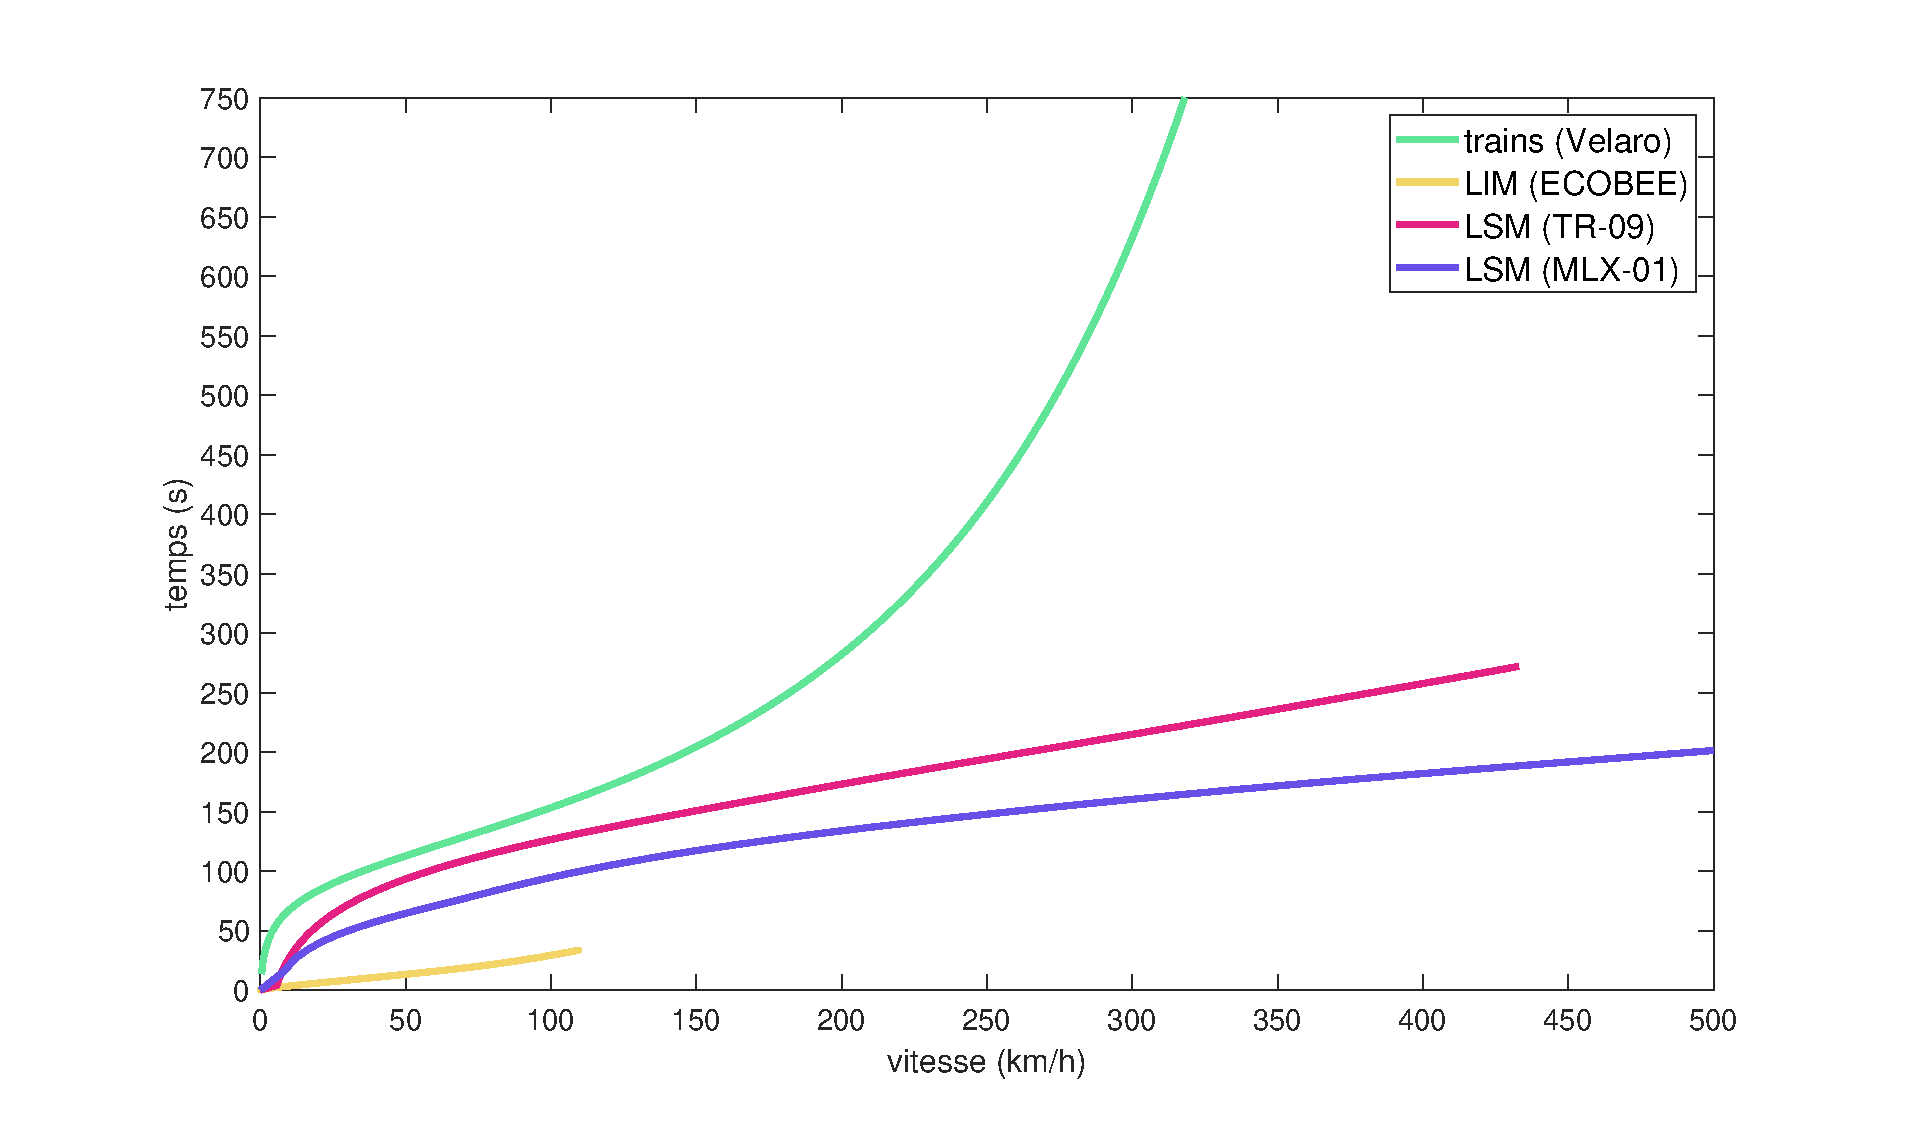
\includegraphics{./fig/TP.eps}}
  \label{temps perdu}
  \caption{time lost per stop as a function of speed\cfannexe{3}}
\end{figure}



\pagebreak %page 11
\tab At low speeds ($V<120 km/h$), it can be noticed that the vehicle losing the least time is the LIM, which can be explained by its strong accelerations and decelerations that remain very high regardless of the train travel speed. \\
\linebreak
\tab At high speeds, it is easy to see that LSM vehicles are much more efficient than trains, having for example an average lost time of 190 seconds for a speed of 300km/h against 635 seconds for the Velaro, that is to say a significant gain of 445 seconds (or 7 minutes and 25 seconds) per stop.
However, the data can change significantly from one vehicle to another for the same technology, as between the SCmaglev and the transrapid.
Moreover, the average time lost per stop is dependent on potential speed steps between different types of lines. \\
\linebreak
\tab We can observe that in addition to having very high attainable speeds, LSM vehicles have high deceleration and acceleration capacities, superior to trains, making them the best guided transport in terms of travel time.
As for LIM, although the attainable speeds are lower than those of trains, the decelerations and accelerations are still higher than those of trains, allowing time savings on routes with more stops.
Thanks to their capacities, maglev vehicles would therefore allow a significant time saving on routes with frequent stops. \\



\pagebreak %page 12
\subsection{Cost}
\tab After discussing the route and its importance to the user, we turned to the builder's perspective.
For the builder, the total cost of a line is a primary factor in planning the line.
This section will discuss all aspects that have a major impact on the cost, from construction to maintenance to energy consumption.

\begin{addmargin}[30px]{0px} \subsubsection*{Construction cost}\end{addmargin}
\tab The cost of infrastructure and roads is one of the most important points when choosing a mode of transport from the manufacturer's point of view.
Rail infrastructure is known to be expensive, so it is important to position maglev on this point. \\
\linebreak
\tab For LIM technologies, it is interesting to ask whether the similarities of the system will keep the cost low.
In a 2018 report by the European Commission, the cost per kilometer of conventional train lines in Europe is estimated at 8.8 $\pm$ 1.7M \euro/km\bettercite{coutkmtrain}.
Looking at the existing LIM lines, the cost per kilometer is estimated at 43.7 ± 4.8M \euro/km\cfannexe{1}.
This value is still 5 times higher than the cost per kilometer of a conventional line. \\
\linebreak
\tab For the LSM lines, the observation is similar.
To obtain a closer comparison, we are interested in High Speed Lines.
In France, the average cost per kilometre of the last high-speed lines built was 16M \euro/km\bettercite{coutkmlgv}, which remains within the European average of 14.5 ± 2.5M \euro/km\bettercite{coutkmtrain}.
As for the cost per kilometer of the LSM lines, it is quite difficult to estimate.
Currently only one line is open and a second one is under construction, but their cost per kilometer varies greatly.
The cost of the Chuo Shinkansen line is extremely high and easily exceeds 200M \euro/km\cfannexe{1}  because the area on which it is built is mountainous, forcing it to be mostly underground (86\% of the route is in tunnels\bettercite{chuoshinkansen}).
Thus, the cost of the Chuo Shinkansen line is not representative of the potential cost per kilometer of an outdoor line.
With the numerous researches made on LSM technologies and more particularly on Transrapid (rolling stock of Shanghai maglev express line), it is estimated that the cost per kilometer of future lines would be close to 36.6M \euro/km\cfannexe{1}. \\
\linebreak
\tab Although the cost per mile of LIM lines is at first glance higher than that of LSM lines, it is important to point out that LSM technologies have been much more studied.
LIM technologies still have good potential for cost reduction if further research on the technologies is conducted.
Some projects are even forecasting mileage costs as high as 18M \euro/km\bettercite{coloradomaglev} and the costs of more recent lines tend to approach this estimate rapidly, as is the case with the line built by the company Xinzhu in Chengdu, China\cfannexe{1}. \\
\tab In addition, LSM lines have a major drawback when the ridership of a line increases, as it is impossible to increase the frequency of trains if the line has not been properly sized.
It is therefore essential to properly size the lines, while remaining cautious about a potential explosion in manufacturing and maintenance costs. \\
\tab Considering this new estimate for LIM technologies, the results are logical considering the technologies involved.
The strong increase in cost for LSM technologies is mainly due to the complexity and ubiquity of the technologies.
As these technologies are mostly located on the track, the costs are based on distance and not on ridership (although ridership remains a key point to consider when creating an LSM line).
These lines require a high frequency of collection, and very precise technologies (remember that LSM vehicles go at speeds exceeding 500 km/h), so the price increases drastically. \\

\pagebreak % page 13
\begin{addmargin}[30px]{0px} \subsubsection*{Energy consumption}\end{addmargin}
\tab Energy consumption is an important factor to consider.
Since our study only deals with electric and catenary powered trains and both maglev technologies are also catenary powered (the catenary is located under the rail or inside the rail), we will only focus on the energy intensity.
The energy intensity is an important factor when choosing a transport system, it allows to calculate the energy needed for its operation, independently of the characteristics and auxiliary consumptions (lighting, heating, ...). It is calculated : \\
\begin{itemize}
  \item By looking at the energy required to move a vehicle seat over a distance of one kilometer (expressed in Wh/step-km),
  \item By looking at the energy required to move one square meter of the vehicle over a distance of one kilometer (expressed in Wh/m²-km).
\end{itemize}
\tab We will use the second measure because it is independent of the traction program (mainline or regional), and of the potential advantages linked to the gauge (double-deck cars).

\begin{figure}[H]
  \centering
  \scalebox{0.5}
  {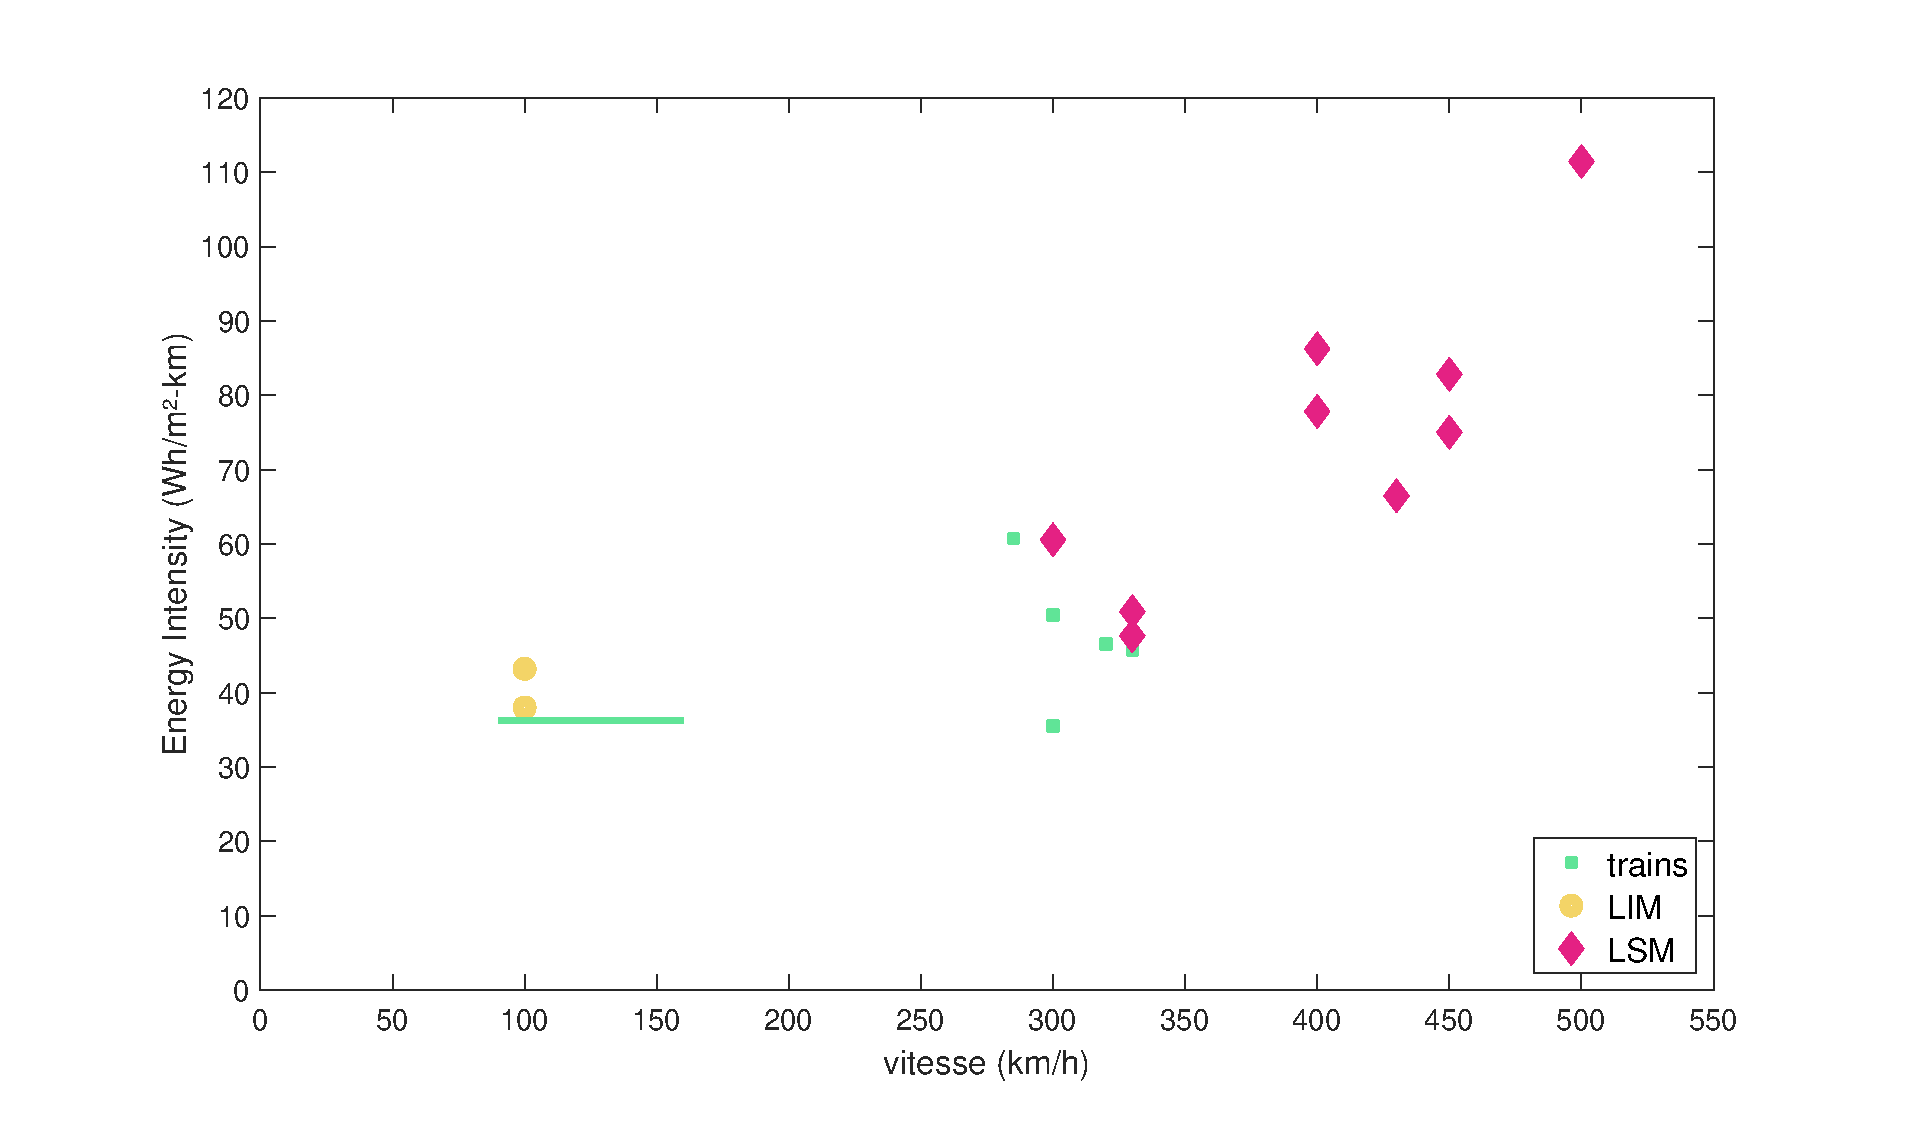
\includegraphics{./fig/EI.eps}}
  \label{energy intensity}
  \caption{Energy intensity by speed and technology\bettercite{linimo}{ei}{railwayhandbook}}
\end{figure}



\pagebreak %page 14
\tab When comparing trains and maglev technologies at a commercial speed of 300-330 km/h, maglev technologies appear to be just as efficient as wheel-rail technologies, with the only variations being in the points mentioned above.
The similarity of the results obtained between the different technologies can be explained in two points:
\begin{itemize}
  \item First, using Newton's first law applied to trains, we can see that at constant speed, the only energy consumption (excluding auxiliaries) is to counter the resistive forces, which remain in the same order of magnitude for the different technologies\bettercite{ei},
  \item Second, the traction chain efficiencies of the technologies remain very high.
\end{itemize}

\tab Indeed, the train drive train is known to be very efficient.
The efficiency of this one starting at 78\% for very low speeds and quickly exceeding 90\% for high speeds\bettercite{thesetgv}.
Maglevs equipped with LSM motors have the advantage of the EDS levitation system.
These have an efficiency very close to that of the train traction chain with values ranging from 80\% to 85\% and up to 92\% by optimizing the length of the track sections\bettercite{coloradomaglev}. \\
\linebreak
\tab If we look at very high speeds, we see an increase in Energy Intensity, which is consistent with the fact that for high speeds, the resistive forces increase with the square of the speed.
Taking these different points into consideration, the increase in consumption on the LSM lines is not alarming.
The measurement performed on the rolling stock of the Chuo Shinkansen line (MLX-01 or SCmaglev) at 500km/h may be an overestimation because of the test conditions, performed in tunnels where the resistant forces are higher. \\
\linebreak
\tab For low speeds, the observation remains similar.
There are no major differences between trains and maglevs with LIM engines.
However, the tests on LIM lines are still low and the indicated values could change with future research.
Comparing these two technologies in a similar way, we could think that the energy intensity of LIM systems would remain higher than that of trains for the same speeds, the efficiency of LIM systems being estimated between 70\% and 77\%\bettercite{coloradomaglev}.
Therefore, more input energy would be required to counteract these losses caused by magnetic leakage, due to the air gap (gap between the rail and the vehicle). \\
\linebreak
\tab Therefore, more energy would have to be supplied. It can be concluded that energy consumption during travel is not a decisive factor in the choice of the guided vehicle technology.
The evolution of this factor during the last 50 years and its potential evolution in the future years remains weak\bettercite{transportationenergy} ; so it will still not have an impact.



\pagebreak %page 15
\begin{addmargin}[30px]{0px} \subsubsection*{Maintenance}\end{addmargin}

\tab In the case of a LIM vehicle, the lack of direct contact between the vehicle and the track and the much smaller number of moving parts than for a train result in lower maintenance costs and a longer service life.
For an LSM vehicle, despite the absence of direct contact between the vehicle and the track and the reduced number of moving parts, maintenance costs are very high due to the highly developed, complex and expensive technologies along the track.
In addition, the track is subject to extreme electromagnetic stresses at a very high frequency, requiring increased maintenance. \\
\linebreak
\tab However, the maintenance costs of maglev vehicles remain higher than those of a train due to the low implementation of these lines and therefore the low number of spare parts.
These parts are sometimes no longer produced and therefore need to be produced again, as for example for the LINIMO. \\
\linebreak
\linebreak
\tab The costs required to build the lines as well as to maintain them and the vehicles show a strong difference between train and maglev vehicles.
Thus, comparing LSM lines to HSR lines and LIM lines to conventional train lines, it appears that maglev lines are much more expensive to build.
Regarding line and vehicle maintenance, maglev lines are again more expensive than trains.
However, a decrease in the maintenance costs of LIM lines and vehicles is possible with their development, unlike LSM lines which require a very high maintenance due to the technology of the lines.
Only the energy consumption varies little, keeping the same comparisons.




\pagebreak %page 16
\subsection{Other selection criteria}
\tab After noting the strong performance of maglev technologies in terms of travel time and their high associated costs, it is also important to mention some other points that could be critical when planning a line.

\begin{addmargin}[30px]{0px} \subsubsection*{Ramps}\end{addmargin}
\tab In our application of Newton's first law performed during the acceleration, we issued comparison conditions such that the resistive force R$_p$ is zero.
This term describes the declivity of the track in ramp or slope and is expressed as : \\
$$R_p = Mgi$$
with: \\
\begin{itemize}
  \item i the angle in mm/m,
  \item M the mass of the complete vehicle,
  \item g the gravitational acceleration constant.
\end{itemize}
\tab The objective here is to be able to take a maximum ramp (highest i), without having a resistive force that is too constraining.
To maximize the attainable ramps, we must again maximize the traction effort or minimize the mass of our rolling stock. \\
\linebreak
\tab Taking again the data of the acceleration section on the mass per unit area (830 kg/m², 820 kg/m² and 650 kg/m² respectively for HSR, LIM and LSM) as well as their length (from 200m or 450m, 80m to 120m and 30m to 50m respectively for HSR, LIM and LSM), we find that the train is much more disadvantaged on the displaced mass than the two maglev technologies, due to its high mass per unit area and its length
Looking at the existing lines we find the following results: \\
\begin{itemize}
  \item i$_{train}$ between 30\textperthousand and 35\textperthousand
  \item i$_{LIM}$ between 60\textperthousand and 70\textperthousand\bettercite{incheonairport}
  \item i$_{LSM}$ around 40\textperthousand\bettercite{chuoshinkansen} (Result on the Chuo Shinkansen line)
\end{itemize}

\tab The above results make sense in view of the powers involved.
However, it is important to specify that the gradient results for the train and LIM are realized in degraded mode (at reduced speed), while the shinkansen line is in strongly graded areas, the ramps remain low to preserve a high speed.
Considering as for the other technologies a degraded mode, the traversable gradients for LSM lines would be about  100 \textperthousand \:to 120 \textperthousand\cfannexe{2}\bettercite{maglevus}.



\pagebreak %page 17
\begin{addmargin}[30px]{0px} \subsubsection*{Radius of curvature and cant}\end{addmargin}
\tab For safety reasons, the radius of curvature is an important point in the plan of a maglev train or vehicle. \\
In the case of a LIM vehicle, for a speed of 80 km/h, the average radius of curvature varies between 500 and 800 meters\bettercite{incheonairportev}{changshadata} \, depending on the line.
As for the train, for this same speed the average radius of curvature is only 350 m\bettercite{thesetgv}.
For LSM vehicles, for much higher speeds of 400 km/h and 500 km/h, it is respectively 4200 and 6500 m\bettercite{rayonLSM}, against 5500 m for a train at 350 km/h\bettercite{thesetgv}. \\
\linebreak
For comfort and safety reasons, the vertical acceleration in curves does not exceed +0.1g and the transverse acceleration does not exceed 0.03g\bettercite{deversLSM}.
To decrease these values, the radius of curvature can be increased or a cant can be added.
For the same radii and speeds as above and considering an can deficiency, a cant angle of about 3° is obtained for the LIM\bettercite{changshadata} \, against 6° for the train and 15° for the maglev LSM\bettercite{deversLSM}.
Since LIM vehicles are mainly urban vehicles, a higher radius of curvature is required than for a train for comfort reasons.
In the case of LSM vehicles, the higher superelevation allows for a smaller radius of curvature than for trains. \\

\begin{addmargin}[30px]{0px} \subsubsection*{Impact of weather conditions}\end{addmargin}
\tab A last point to compare is the ability of the technologies to be operational independently of the weather conditions.
Here the wheel-rail contact still shows its weakness.
Trains are known to have a huge delay in low temperatures, as well as in autumn with the leaves falling on the tracks and limiting even more the already weak adhesion of the latter. \\
\tab Maglev technologies eliminate any contact with the rail and maintain their position thanks to an electromagnetic field.
The electromagnetic field is only slightly influenced by the presence of non-metallic objects on the track, and maglev lines are generally elevated, so they are not affected by weather conditions.



\pagebreak %page 18
\section*{Conclusion}
\tab The different points studied allow us to establish the different situations where it is preferable to opt for maglev technologies rather than conventional rail technologies.
Due to the high gradient capabilities of both maglev technologies, it might be preferable to choose them for areas with high gradients.
In addition, the increased acceleration and deceleration capabilities of LIM technologies would allow a reduction of travel times on regional networks where travel time is important.
The same is true for mainline trains with LSM technologies, which have exceptional acceleration and deceleration capacities and very high commercial speeds.
However, the cost per kilometer for the construction of these lines remains three times higher than for conventional high-speed lines, which limits their deployment enormously. \\
\linebreak
\tab It is also important to remember that even if we have found results that best fit our problem, these may remain imprecise due to the multitude of traction programs as well as the weak presence of maglev technologies and the limited amount of research on the subject.
This weak development can be explained by several reasons: \\
\begin{itemize}
  \item First of all, the main countries looking for and developing these systems (Japan, China, Germany,...) are countries with already very developed rail networks. These countries prefer to maintain their existing network and in case they want to develop it, they still prefer to stay on a classical railway system to limit the risks, despite the potential advantages that this system could bring in some cases\bettercite{maglevus}.
  \item In addition, there is a historical reason. The first traces of research on maglev technologies go back to 1908 with a patent filed by Tom.L.JohnSon\bettercite{firstpatent}, with the first tests performed in the 1940s.
\end{itemize}

\begin{figure}[H]
  \label{reseau ferre}
  \centering
  \scalebox{0.48}
  {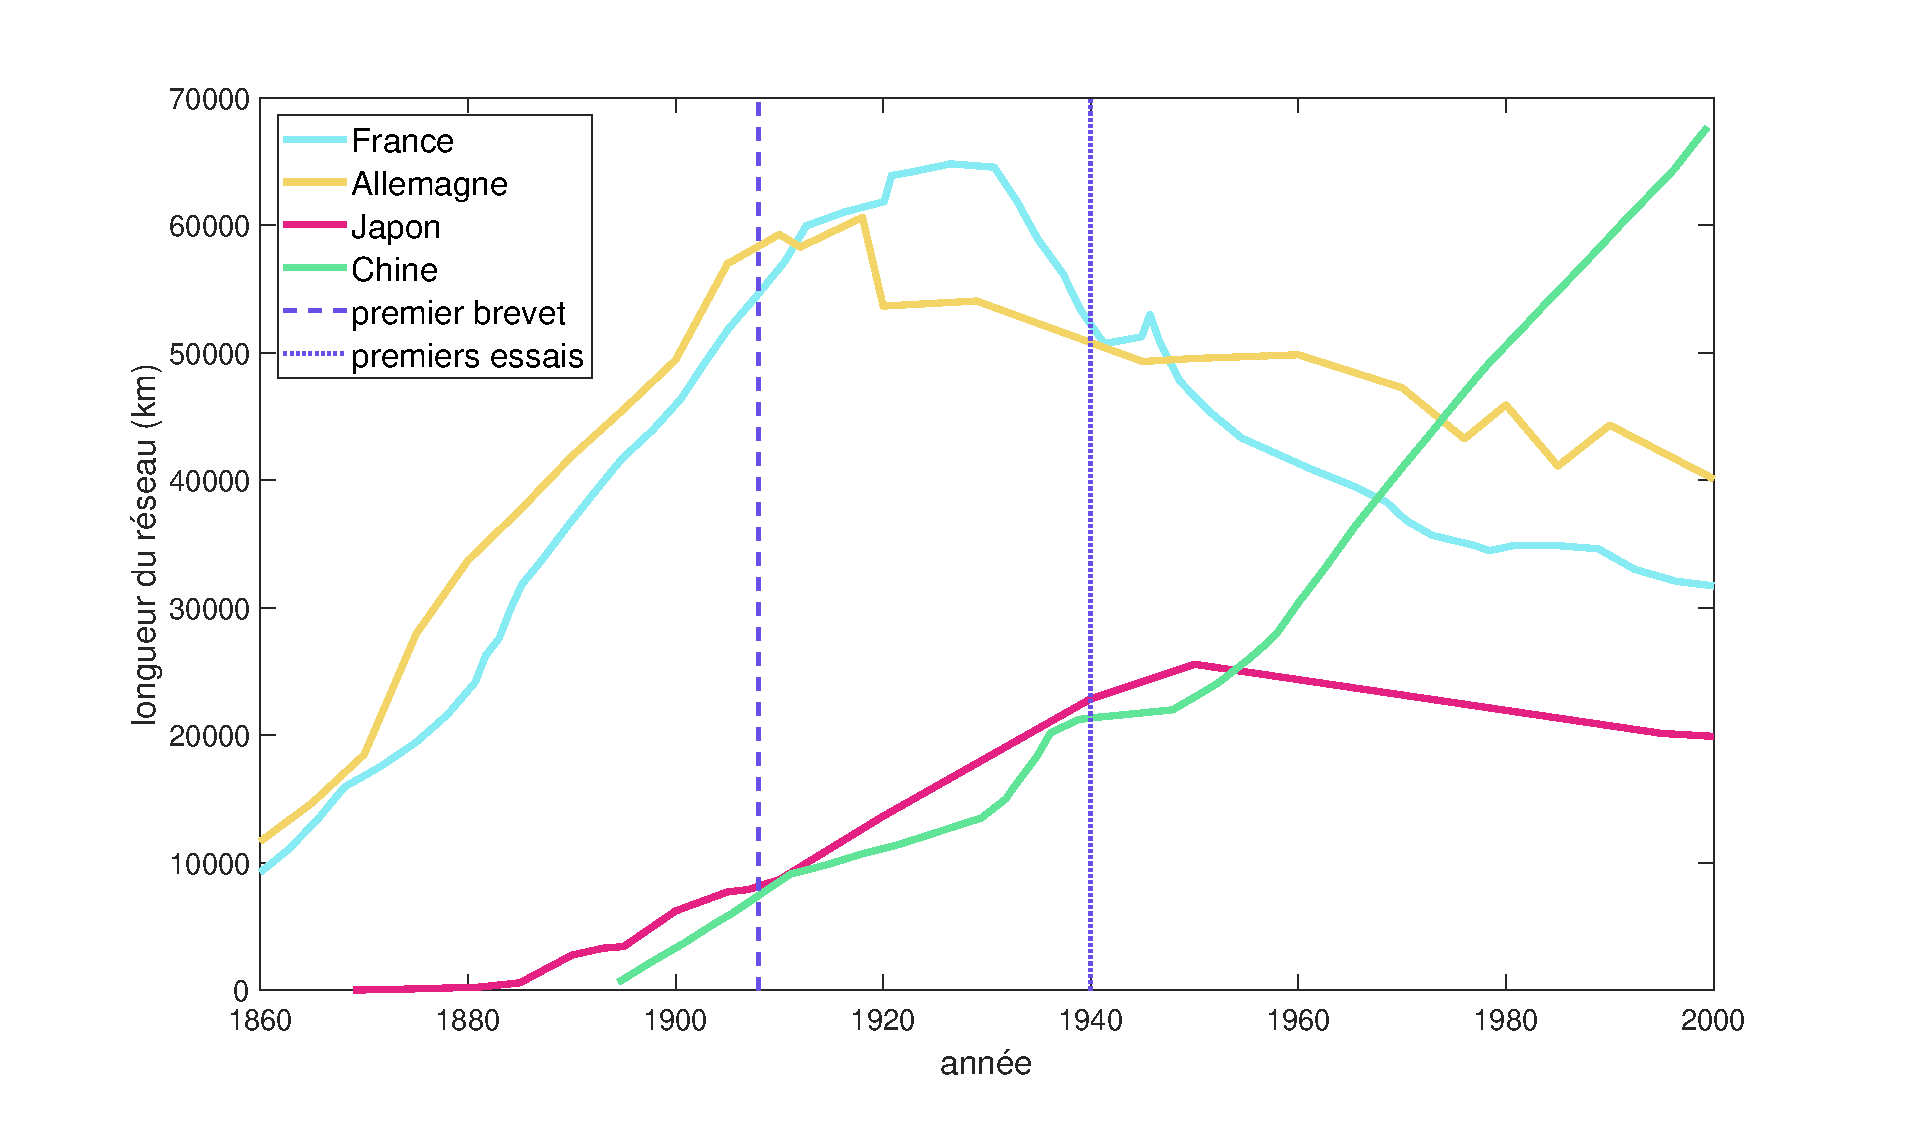
\includegraphics{./fig/RF.eps}}
  \caption{Evolution of the Railways by year\bettercite{rffrance}{rfallemagne}{rfchine}{rfjapon}}
\end{figure}

\pagebreak % Page 20
\begin{addmargin}[30px]{0px}
  The first patent arrived at the height of the development of the various rail networks and the first tests at the peak of their development.
  The researches and applications of these technologies arrived too late in relation to the development of the different railway networks, which explains the current situation of the maglev technologies. \\
\end{addmargin}



\pagebreak %page 20
\begin{appendix}
  \section{Appendices}
  \subsection{Appendix 1: List of lines open or under development}
  \label{annexe 1}

  \bgroup
  \def\arraystretch{1.2}
  \begin{adjustwidth}{-40px}{-40px}
    \begin{tabular}{|c|c|c|c|c|c|c|}
      \hline
      ligne                                                                                & country         & length & speed & cost        & levitation & propulsion \\
      \hline
      Shanghai Transrapid                                                                  & China        & 30.5 km  & 430km/h & 1077M\euro  & EDS + EMS    & LSM        \\
      \hline
      Changsha Express\bettercite{changshadata}{changshasources}                           & China        & 18.5km   & 120km/h & 607M\euro   & EMS          & LIM        \\
      \hline
      Line S1 Beinjing                                                                     & China        & 10km     & 110km/h & ?           & EMS          & LIM        \\
      \hline
      Chengdu Xinzhu                                                                       & China        & 4.5km    & 160km/h & 86M\euro    & EMS          & LIM        \\
      \hline
      UTM-02 Daejeon\bettercite{koreamaglevprogram}                                        & South Korea & 1km      & 100km/h & ?           & EMS          & LIM        \\
      \hline
      Incheon Itl Airport\bettercite{koreamaglevprogram}{incheonairport}{incheonairportev} & South Korea & 6.1km    & 80km/h  & 187M\euro   & EMS          & LIM        \\
      \hline
      Nagoya Linimo\bettercite{linimo}                                                     & Japan        & 8.9km    & 100km/h & 466M\euro   & EMS          & LIM        \\
      \hline
      Chuo Shinkansen\bettercite{chuoshinkansen}                                           & Japan        & 285.6km  & 500km/h & 55000M\euro & EDS + wheels  & LSM        \\
      \hline
    \end{tabular}
  \end{adjustwidth}
  \egroup



  \pagebreak %page 21
  \subsection{Appendix 2: Effort-Speed diagrams}
  \label{annexe 2}
  \begin{figure}[H]
    \label{effort vitesse train}
    \centering
    \scalebox{0.51}
    {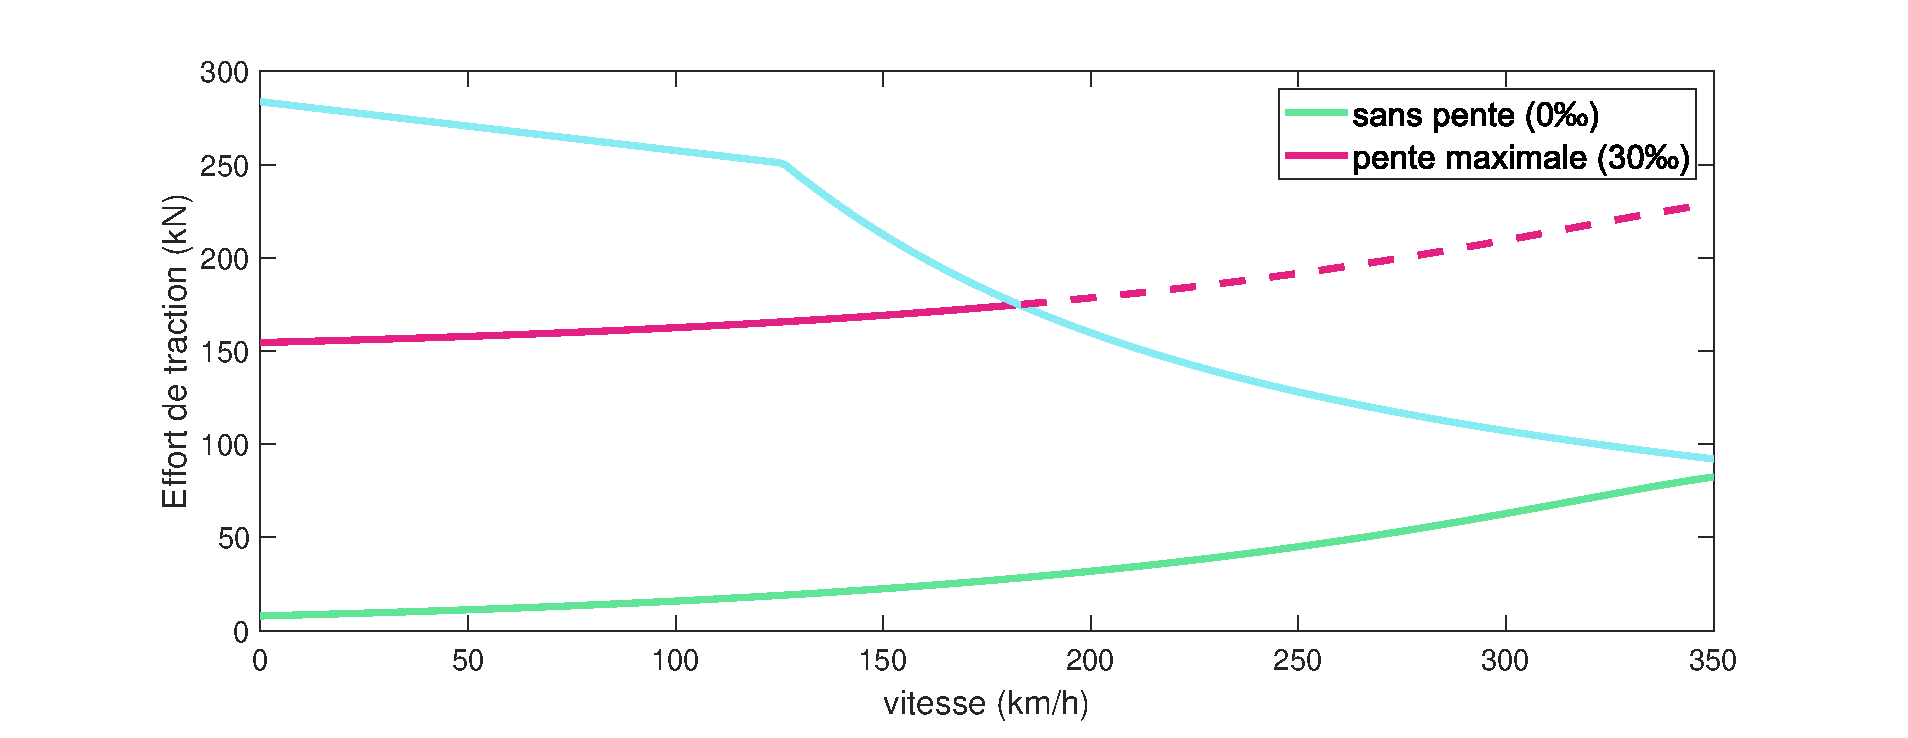
\includegraphics{./fig/EVtrain.eps}}
    \caption{Velaro effort-speed diagram (high-speed self-propelled vehicle)\bettercite{maglevus}}
  \end{figure}

  \begin{figure}[H]
    \centering
    \label{effort vitesse LIM}

    \scalebox{0.51}
    {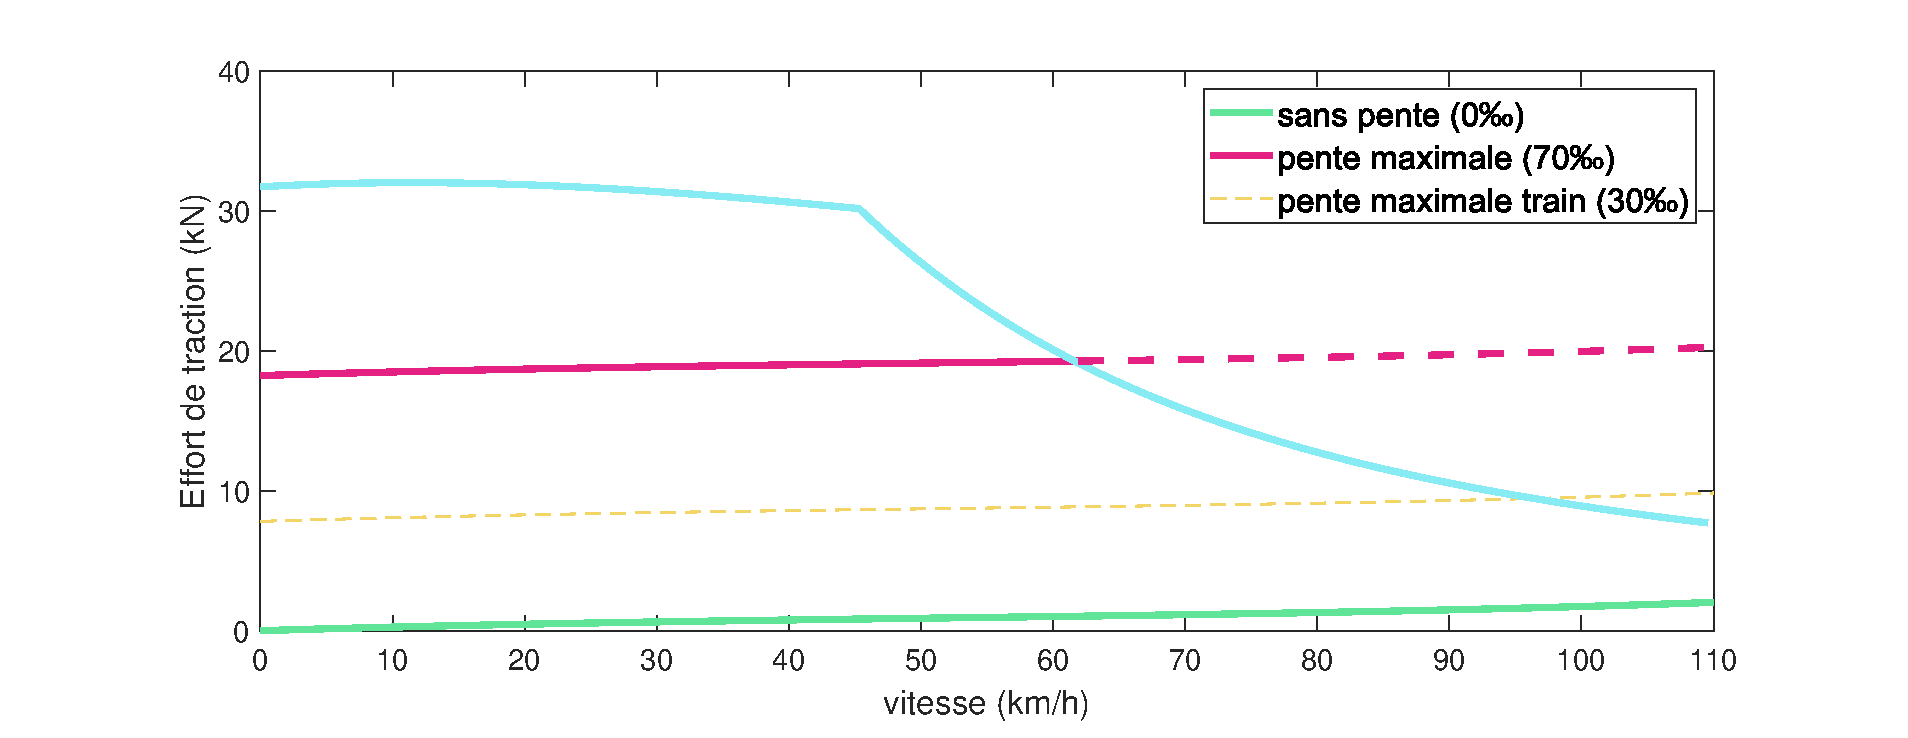
\includegraphics{./fig/EVLIM.eps}}
    \caption{ECOBEE effort-speed diagram (LIM : Incheon International Airport)\bettercite{incheonairportev}}

  \end{figure}
  \begin{figure}[H]
    \centering
    \label{effort vitesse LSM}

    \scalebox{0.51}
    {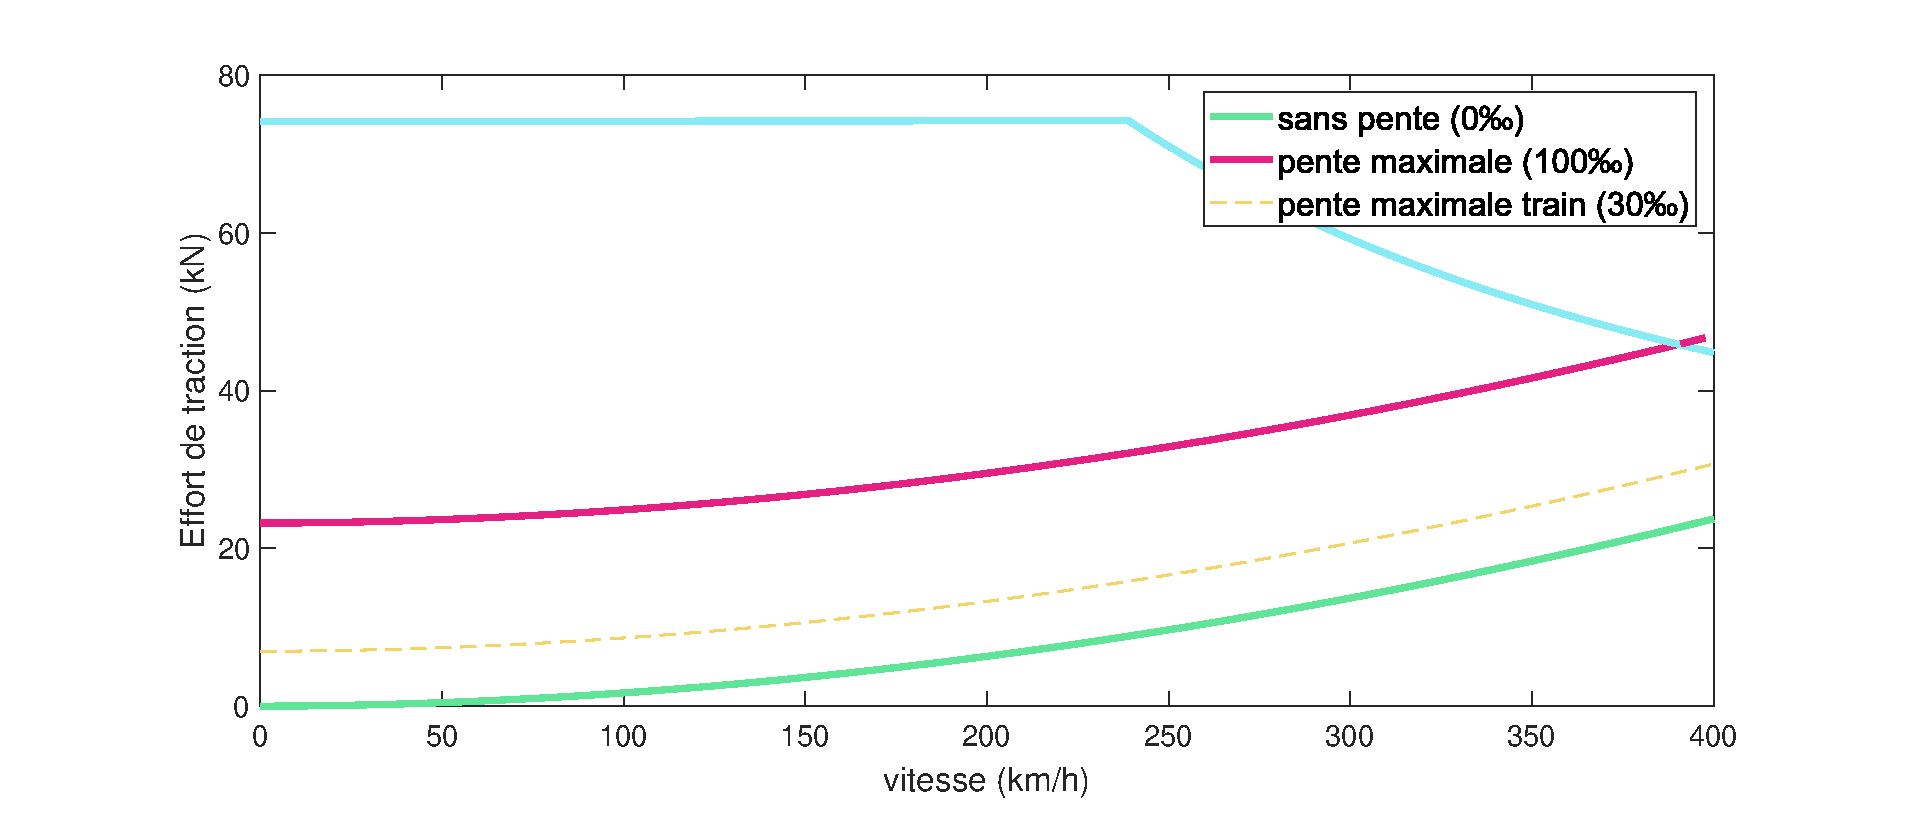
\includegraphics{./fig/EVLSM.eps}}
    \caption{TR-09 effort speed diagram (LSM : Shanghai maglev Express)\bettercite{maglevus}}
  \end{figure}



  \pagebreak % page 22
  \subsection{Appendix 3 : speed-time and speed-distance diagram}
  \label{annexe 3}

  \begin{figure}[H]
    \centering
    \begin{minipage}[H]{0.49\textwidth}
      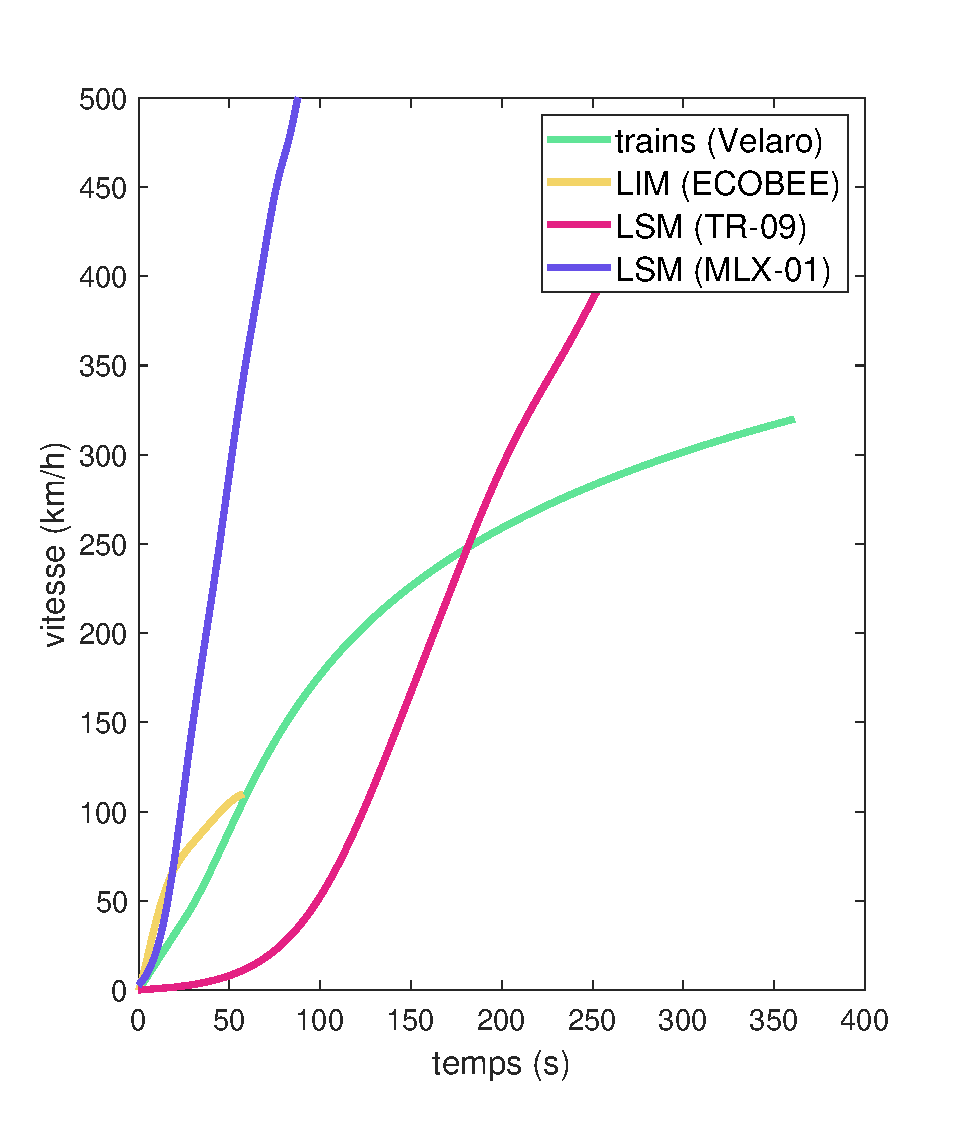
\includegraphics[width=\textwidth]{./fig/Atv.eps}
    \end{minipage}
    \hfill
    \begin{minipage}[H]{0.49\textwidth}
      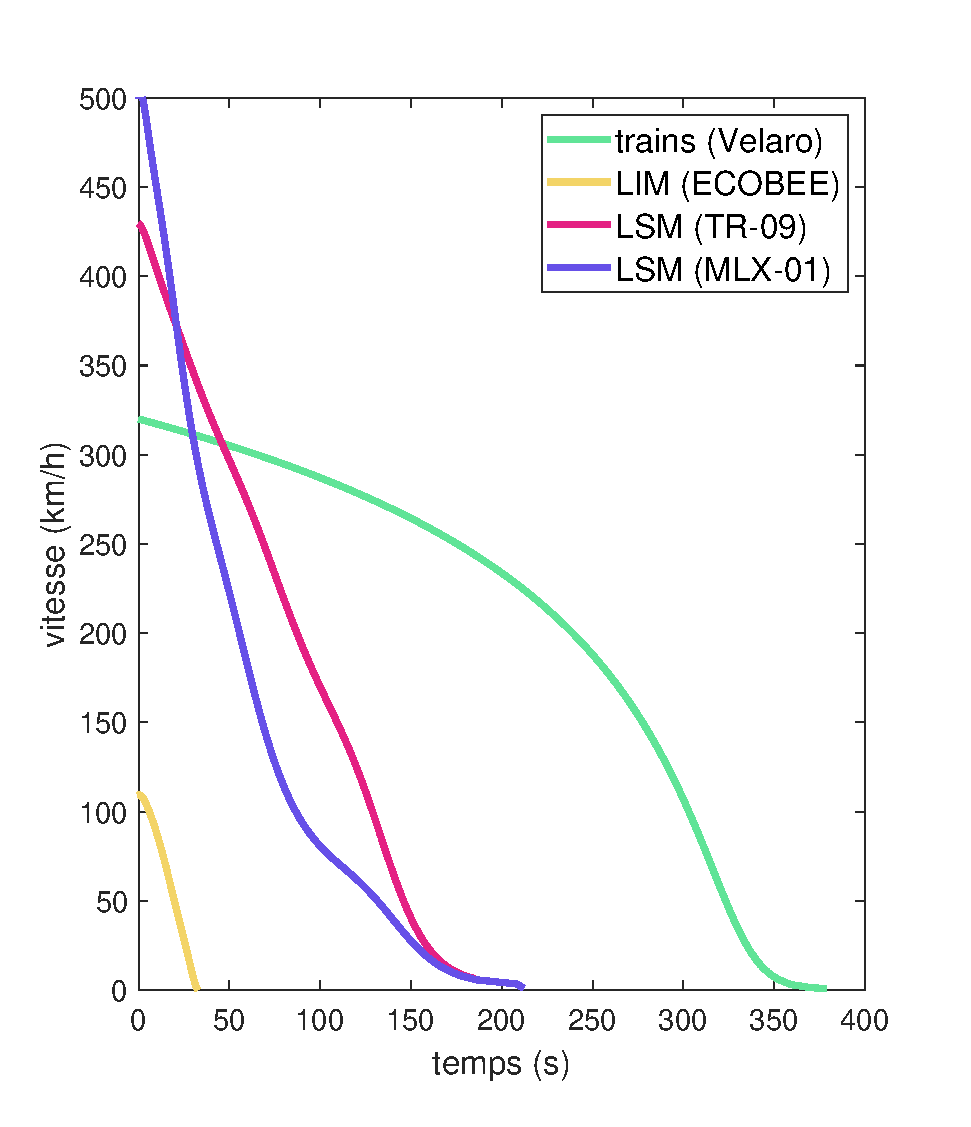
\includegraphics[width=\textwidth]{./fig/Dtv.eps}
    \end{minipage}
    \caption{speed-time diagrams in acceleration and deceleration\bettercite{maglevus}{courbeslimlsm}{incheonairportev}}

    \begin{minipage}[H]{0.49\textwidth}
      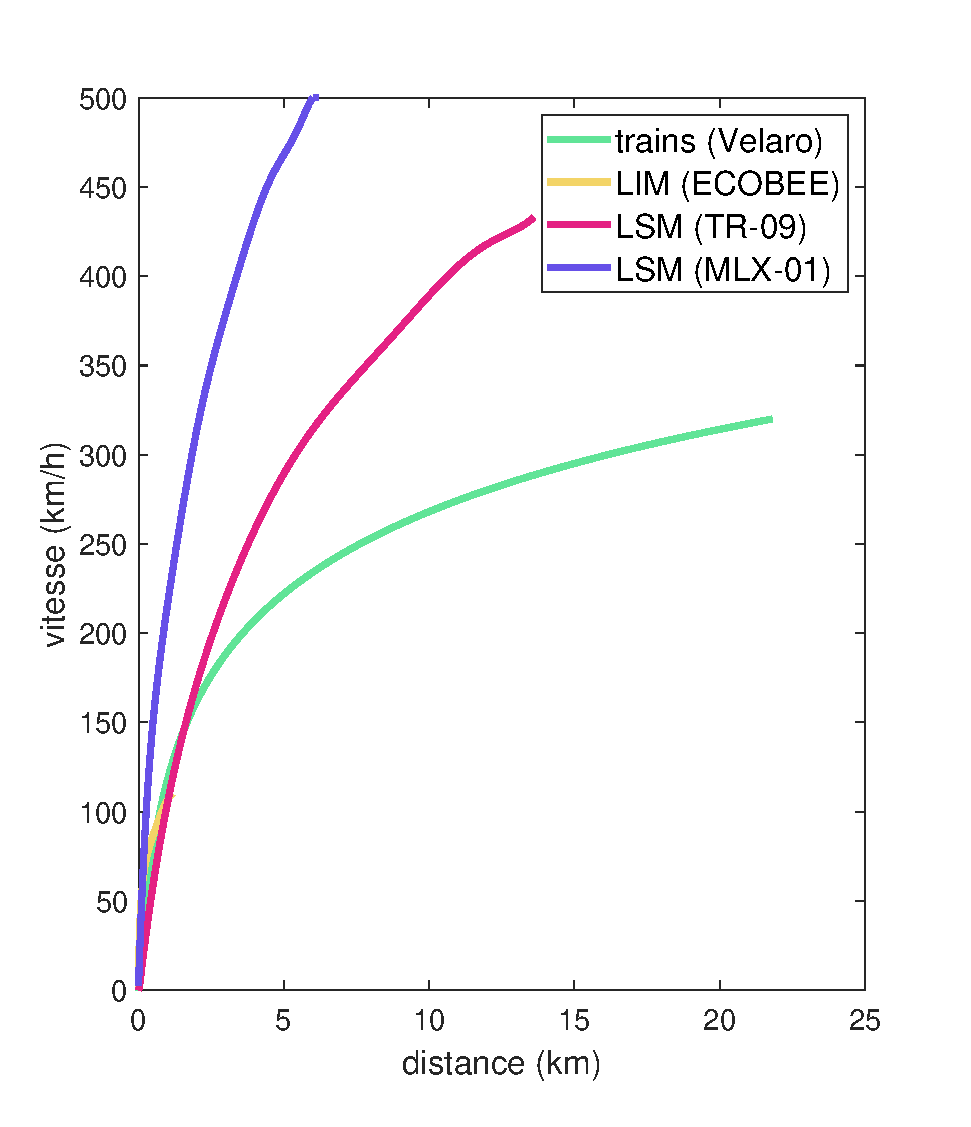
\includegraphics[width=\textwidth]{./fig/Adv.eps}
    \end{minipage}
    \hfill
    \begin{minipage}[H]{0.49\textwidth}
      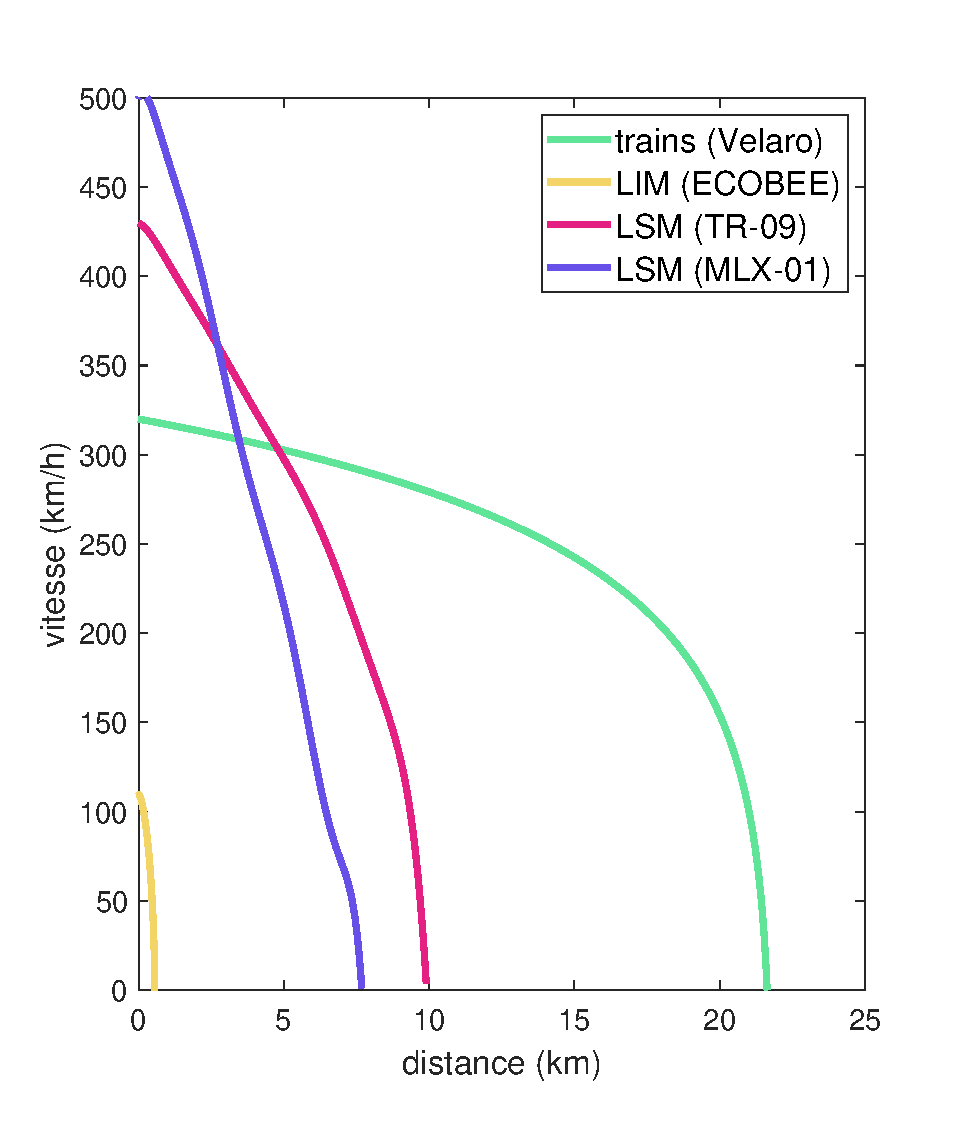
\includegraphics[width=\textwidth]{./fig/Ddv.eps}
    \end{minipage}
    \caption{speed-distance diagrams in acceleration and deceleration\bettercite{maglevus}{courbeslimlsm}{incheonairportev}}
  \end{figure}

\end{appendix}



\pagebreak %sources
\bibliographystyle{unsrt}
\bibliography{sources.bib}
\nocite{*}
\end{document}